\section{Image Filters} \label{s:filters}
	The proper selection of filters is important to the overall effectiveness of the algorithm. As previously mentioned, the intention of DRAGONFIST is to improve a machine learning model's resiliency against adversarial noise. Based on the work done by \citeauthor{goodfellow2015} \cite{goodfellow2015}, adversaries can target specific pixels in an image to which noise will be applied. As such, filters which combine the values of pixels with their neighbours are intuitively more desirable as they increase the difficulty of intoducing noise to specific areas of the image. Therefore, the following filters were considering when designing DRAGONFIST:
	\begin{multicols}{2}
		\begin{itemize}
			\item Edge detection
			\item Gaussian
			\item Average rows
			\item Average columns
			\item Rank
			\item Maximum
			\item Minimum
			\item Median
		\end{itemize}
	\end{multicols}

	\subsection{Descriptions} \label{s:filters:descriptions}
		In order to understand what the filters are doing to the images, a brief explanation of each is given.

		\subsubsection{Edge detection} \label{s:filters:descriptions:edgeDetection}
			The edge detection filter uses the Python library \codeword{skimage.filters.sobel} \cite{skikitImage}. This filter locates and isolates the edges of objects found in an image. An example of this filter applied to images in the MNIST Fashion database \cite{zalandoresearchFashionMNIST} can be seen in Appendix \ref{a:filters} Figure \ref{a:filters:edgeDetection}.

		\subsubsection{Gaussian} \label{s:filters:descriptions:gaussian}
			The Gaussian filter uses the Python library \codeword{skimage.filters.gaussian} \cite{skikitImage}. This filter convolves the image with a Gaussian function to create a ``blurring'' effect. An example of this filter applied to images in the MNIST Fashion database \cite{zalandoresearchFashionMNIST} can be seen in Appendix \ref{a:filters} Figure \ref{a:filters:gaussian}.

		\subsubsection{Average Rows} \label{s:filters:descriptions:averageRows}
			The average rows filter was created by us for this project. This filter finds the average pixel value (i.e. intensity for black and white images and RGB values for colour images) and sets all values in the row to the average. An example of this filter applied to images in the MNIST Fashion database \cite{zalandoresearchFashionMNIST} can be seen in Appendix \ref{a:filters} Figure \ref{a:filters:averageRows}.

		\subsubsection{Average Columns} \label{s:filters:descriptions:averageCols}
			The average columns filter was created by us for this project. This filter works similarly to the average rows filter described in Section \ref{s:filters:descriptions:averageRows} though is applied to an image's columns instead of rows. An example of this filter applied to images in the MNIST Fashion database \cite{zalandoresearchFashionMNIST} can be seen in Appendix \ref{a:filters} Figure \ref{a:filters:averageCols}.

		\subsubsection{Rank} \label{s:filters:descriptions:rank}
			The rank filter uses the Python library \codeword{scipy.ndimage.rank_filter} \cite{scipy}. This filter scans over an image with a rectangle (a 3x3 square was used in this project) and creates a histogram of the pixel values in the rectangle. One value in this histogram is then chosen to be applied to every pixel in the rectangle (a random value in the histogram was chosen for this project's rank filter). An example of this filter applied to images in the MNIST Fashion database \cite{zalandoresearchFashionMNIST} can be seen in Appendix \ref{a:filters} Figure \ref{a:filters:rank}.

			If the last value is chosen, a maximum filter is created. An example of this filter applied to images in the MNIST Fashion database \cite{zalandoresearchFashionMNIST} can be seen in Appendix \ref{a:filters} Figure \ref{a:filters:max}.

			If the first value is chosen, a minimum filter is created. An example of this filter applied to images in the MNIST Fashion database \cite{zalandoresearchFashionMNIST} can be seen in Appendix \ref{a:filters} Figure \ref{a:filters:min}.

			If the center value is chosen, a median filter is created. An example of this filter applied to images in the MNIST Fashion database \cite{zalandoresearchFashionMNIST} can be seen in Appendix \ref{a:filters} Figure \ref{a:filters:median}.

	\subsection{Filter accuracy} \label{s:filters:accuracy}
		When applying each filter to the system, it is important to remember the overall goal of the model -- to accurately classify its input. Therefore, each filter's accuracy in classification is important to consider to ensure the overall model maintains a high accuracy as well. Each filter was tested individually in order to determine its classification accuracy. The results of these tests can be observed in Table \ref{t:filterAccuracies}. All filters were trained using the same, standardized model architecture on the MNIST Fashion database \cite{zalandoresearchFashionMNIST} which contains \(60000\) images.

		Almost all filters demonstrated high accuracies except for the averaging filters. This was expected as these filters destroy much of the image's data which makes it harder to classify on the image later on; however, the filters were chosen to be included in the project as they combine a large amount of the image's pixels which intuitively makes it more difficult to target single pixels for adversarial noise.
		\begin{table}
			\begin{center}
				\caption{Image filter accuracies.}
				\label{t:filterAccuracies}
				\begin{tabular}{l|l}\hline
					\textbf{Filter} & \textbf{Accuracy (\(\%\))}\\\hline
					Identity & 91.57\\\hline
					Edge detection & 90.24\\\hline
					Gaussian & 90.07\\\hline
					Average rows & 79.66\\\hline
					Average columns & 82.09\\\hline
					Rank & 88.62\\\hline
					Maximum & 90.07\\\hline
					Minimum & 88.76\\\hline
					Median & 88.62\\\hline
				\end{tabular}
			\end{center}
		\end{table}

		These accuracies vary based on the number of epochs over which the model is trained. The accuracies of the mentioned filters for model over varying epochs can be seen in Figure \ref{f:filters:accuracies}.
		\begin{figure*}
			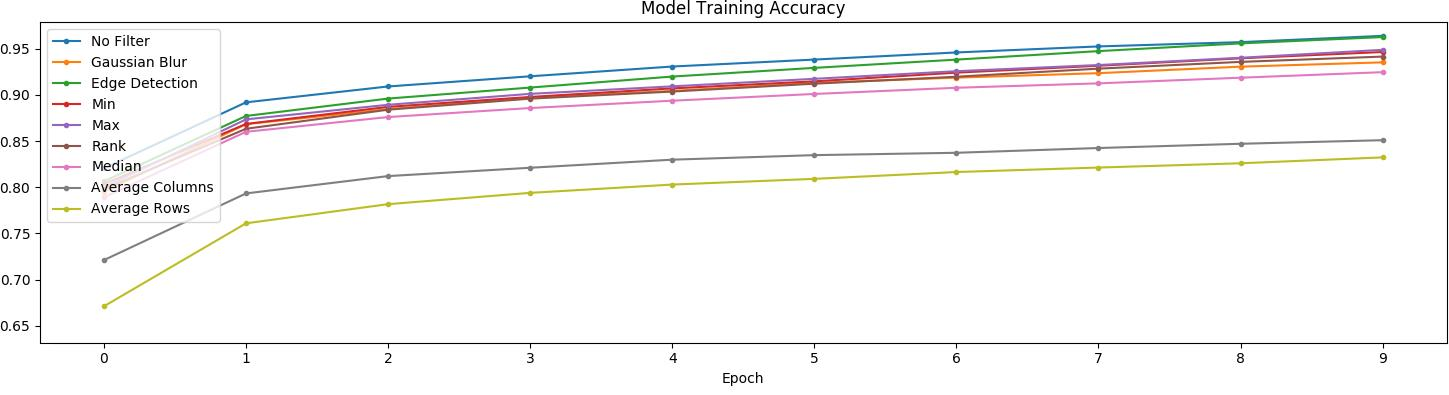
\includegraphics[width=\linewidth]{filter-accuracies.jpeg}
			\caption{Classification accuracy during training for various image filters.}
			\label{f:filters:accuracies}
		\end{figure*}

	\subsection{Filter selection} \label{s:filters:selection}
		As previously mentioned, filters were selected for use in the DRAGONFIST model based on their intuitive ability to combine data from neighbouring pixels in order to increase the difficulty of targetting specific pixels with adversarial noise. Due to time constraints, a more systematic approach to filter selection could not be created. As such, we leave this to potential future research. Tools which test a filter's ability to defend against adversarial noise could help identify filters which would improve DRAGONFIST's ability to mitigate attack and would be extremely useful for this project.
